\documentclass[12pt,a4paper]{article}

% Packages
\usepackage[margin=0.9in]{geometry}
\usepackage{times}          % Times New Roman
\usepackage{graphicx}
\usepackage{booktabs}
\usepackage{caption}
\usepackage{subcaption}
\usepackage{hyperref}
\usepackage{float}
\usepackage{enumitem}
\usepackage{xcolor}
\usepackage{amsmath}
\usepackage{url}
\usepackage{setspace}

\singlespacing
\setlength{\parskip}{4pt}
\setlength{\parindent}{0pt}

\hypersetup{
    colorlinks=true,
    linkcolor=blue,
    citecolor=blue,
    urlcolor=blue
}

\begin{document}

% ============================================================
% Title
% ============================================================
\begin{center}
    {\LARGE\bfseries VecBench-EC2: Performance Benchmarking of Open-Source\\
    Vector Databases for RAG Systems on AWS EC2}\\[12pt]
    {\large CS5296 Cloud Computing, Spring 2026 --- Technical Project}\\[8pt]
    {\large Group 666}\\[6pt]
    QING Qiguo (59905956) \quad LUO Yuxi (59570433)\\[4pt]
    Department of Computer Science, City University of Hong Kong
\end{center}

\vspace{4pt}
\hrule
\vspace{8pt}

% ============================================================
% Abstract
% ============================================================
\section*{Abstract}

Retrieval-Augmented Generation (RAG) systems depend on vector databases for efficient nearest-neighbor search over high-dimensional embeddings. Selecting an appropriate vector database involves trade-offs in ingestion speed, query latency, scalability, and cost. This paper presents VecBench-EC2, a systematic benchmark comparing three open-source vector databases---Milvus, Chroma, and Weaviate---on AWS EC2 using the SIFT1M dataset (128-dimensional vectors). We evaluate ingestion throughput, query latency percentiles (P50/P95/P99), concurrency scaling (1--16 threads), memory consumption, and total cost of ownership (TCO) at three dataset scales (10K, 100K, 1M vectors). All experiments run on a t2.large instance (2~vCPU, 8~GB RAM) under controlled conditions to ensure fair comparison. Our results reveal that Chroma achieves the lowest query latency (3.6~ms average) and highest concurrent throughput (5,479~QPS at 4 threads) at moderate scale, but fails at 1M vectors due to memory exhaustion. Milvus demonstrates superior scalability, handling 1M vectors with 35,370~vec/s ingestion throughput, though it exhibits higher per-query latency (290~ms) due to gRPC overhead. Weaviate offers balanced performance but encounters timeout failures at 1M scale. These findings provide practical guidance for deploying vector databases in resource-constrained cloud environments.

% ============================================================
% 1. Introduction
% ============================================================
\section{Introduction}

The rapid adoption of Retrieval-Augmented Generation (RAG) architectures has elevated vector databases to a critical infrastructure component in modern AI systems~\cite{lewis2020rag}. A RAG pipeline encodes documents into high-dimensional embedding vectors, stores them in a vector database, and retrieves the most relevant vectors at query time to augment language model responses. The choice of vector database directly impacts system latency, throughput, and operational cost.

The vector database market has grown significantly, with both commercial (Pinecone, Zilliz Cloud) and open-source (Milvus, Chroma, Weaviate) solutions competing for adoption~\cite{pan2024survey}. However, practitioners often lack controlled benchmarks to guide their selection, particularly in cloud environments where resource constraints and pricing affect deployment decisions.

This project addresses this gap by benchmarking three popular open-source vector databases on AWS EC2:
\begin{itemize}[nosep]
    \item \textbf{Milvus v2.4}~\cite{wang2021milvus}: A distributed vector database with segment-based architecture, supporting multiple index types (IVF\_FLAT, HNSW, FLAT) and strong consistency via etcd.
    \item \textbf{Chroma (latest)}~\cite{chroma2024}: A lightweight, developer-friendly embedding database designed for rapid prototyping, using an HTTP API.
    \item \textbf{Weaviate v1.24}~\cite{weaviate2024}: A cloud-native vector search engine with a GraphQL/REST API and built-in HNSW indexing.
\end{itemize}

Our benchmarking methodology follows established practices from ANN-Benchmarks~\cite{annbenchmarks} and VectorDBBench~\cite{vectordbbench}, with the following contributions:
\begin{enumerate}[nosep]
    \item A unified Python framework that benchmarks all three databases under identical conditions on the same EC2 instance.
    \item Comprehensive evaluation covering ingestion, query latency percentiles, concurrency scaling, and system resource monitoring.
    \item TCO analysis for deploying vector databases on AWS EC2.
    \item Documentation of scalability limits on memory-constrained instances.
\end{enumerate}

% ============================================================
% 2. Background
% ============================================================
\section{Background and Related Work}

\subsection{Vector Similarity Search}

Vector databases perform approximate nearest neighbor (ANN) search over high-dimensional vectors using distance metrics such as L2 (Euclidean) or cosine similarity. The core challenge is maintaining sub-millisecond query latency as dataset size grows from thousands to millions of vectors. Index structures such as FLAT (brute-force), IVF (inverted file), and HNSW (hierarchical navigable small world)~\cite{malkov2018hnsw} offer different trade-offs between recall accuracy and search speed.

\subsection{Related Benchmarks}

ANN-Benchmarks~\cite{annbenchmarks} evaluates algorithmic performance of indexing libraries (FAISS, Annoy, etc.) but does not benchmark full database systems. VectorDBBench~\cite{vectordbbench} by Zilliz provides a more comprehensive evaluation but targets high-end hardware. Our work fills the gap of benchmarking on resource-constrained cloud instances typical of cost-sensitive deployments, and additionally measures concurrency scaling and TCO.

\subsection{Database Architectures}

Table~\ref{tab:arch} summarizes the architectural differences among the three databases.

\begin{table}[H]
\centering
\caption{Architectural comparison of benchmarked vector databases.}
\label{tab:arch}
\small
\begin{tabular}{lccc}
\toprule
\textbf{Feature} & \textbf{Milvus} & \textbf{Chroma} & \textbf{Weaviate} \\
\midrule
Docker containers & 3 (etcd, minio, standalone) & 1 & 1 \\
API protocol & gRPC & HTTP/REST & REST/GraphQL \\
Default index & FLAT & HNSW & HNSW \\
Storage backend & minio (S3-compatible) & SQLite + Parquet & Built-in LSM \\
Consistency model & Strong/Bounded & Eventual & Eventual \\
\bottomrule
\end{tabular}
\end{table}

% ============================================================
% 3. Methodology
% ============================================================
\section{Experimental Methodology}

\subsection{Fairness Rules}

To ensure a fair comparison, all experiments adhere to the following rules:
\begin{enumerate}[nosep]
    \item Same EC2 instance for every database.
    \item Same OS and Docker version (Ubuntu 22.04, Docker CE latest).
    \item Same dataset (SIFT1M subsets from identical \texttt{.npy} files).
    \item Fixed query set (100 queries randomly sampled from SIFT1M query vectors, seed=42).
    \item Fixed random seed (\texttt{seed=42}) for all operations.
    \item Same \texttt{top\_k=10} for all search benchmarks.
    \item 1-second warm-up pause after initialization.
    \item Each experiment repeated 3 times; results report the mean.
    \item Sequential execution: one database at a time to avoid resource contention.
    \item Fresh state: collection dropped and recreated between rounds.
\end{enumerate}

\subsection{Dataset}

We use the SIFT1M dataset~\cite{jegou2011sift}, a standard benchmark for ANN evaluation containing 1 million 128-dimensional vectors derived from SIFT feature descriptors. We prepare three subsets (10K, 100K, 1M vectors) and a fixed set of 1,000 query vectors, from which 100 are used per benchmark run.

\subsection{Benchmark Framework}

Our Python benchmark framework (\texttt{benchmark.py}) implements a unified \texttt{BaseVectorDB} interface with three adapters (MilvusDB, ChromaDB, WeaviateDB). The framework measures:

\begin{itemize}[nosep]
    \item \textbf{Ingestion}: Batch insert with database-specific batch sizes (Milvus: 10K, Chroma: 5K, Weaviate: object-level batching). Wall-clock time includes index building and flushing.
    \item \textbf{Query latency}: Sequential single-vector queries, recording per-query latency. Percentiles (P50, P95, P99) computed via \texttt{numpy.percentile}.
    \item \textbf{Concurrency}: Multi-threaded query execution using Python's \texttt{ThreadPoolExecutor} at 1, 4, 8, and 16 threads.
    \item \textbf{System metrics}: CPU and memory usage captured via \texttt{psutil} before/after insert and query phases.
\end{itemize}

\subsection{Infrastructure}

\begin{itemize}[nosep]
    \item \textbf{EC2 instance}: t2.large (2 vCPU, 8 GB RAM, burstable)
    \item \textbf{Storage}: 30 GB gp3 EBS volume
    \item \textbf{OS}: Ubuntu 22.04 LTS
    \item \textbf{Docker}: Docker CE with Compose v2
    \item \textbf{Python}: 3.10+ with pymilvus, chromadb, weaviate-client v3
\end{itemize}

% ============================================================
% 4. Results
% ============================================================
\section{Results and Analysis}

\subsection{Ingestion Performance}

Figure~\ref{fig:insert} shows ingestion throughput across the three dataset scales. Key observations:

\begin{figure}[H]
    \centering
    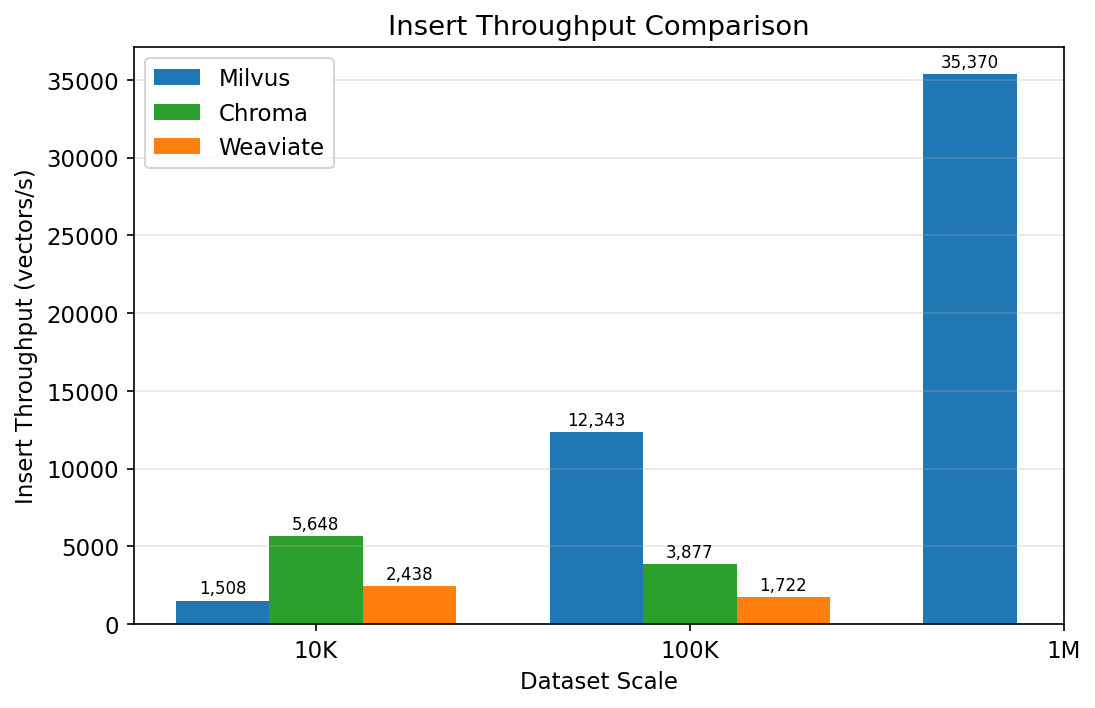
\includegraphics[width=0.78\textwidth]{figures/insert_throughput.png}
    \caption{Insert throughput (vectors/second) by dataset scale. Higher is better.}
    \label{fig:insert}
\end{figure}

\textbf{Milvus} exhibits a counter-intuitive scaling pattern: throughput \emph{increases} from 1,508 vec/s (10K) to 12,343 vec/s (100K) to 35,370 vec/s (1M), because its per-vector amortized cost decreases as collection initialization and index creation overhead is spread over more vectors. \textbf{Chroma} leads at 10K (5,648 vec/s) but degrades to 3,877 vec/s at 100K and fails at 1M due to OOM ($>$5.3 GB). \textbf{Weaviate} shows consistently low throughput (2,438 $\rightarrow$ 1,722 vec/s) due to object-level batching and real-time HNSW index updates.

\subsection{Query Latency}

Figure~\ref{fig:latency} presents query latency distributions at each scale under sequential (1-thread) execution.

\begin{figure}[H]
    \centering
    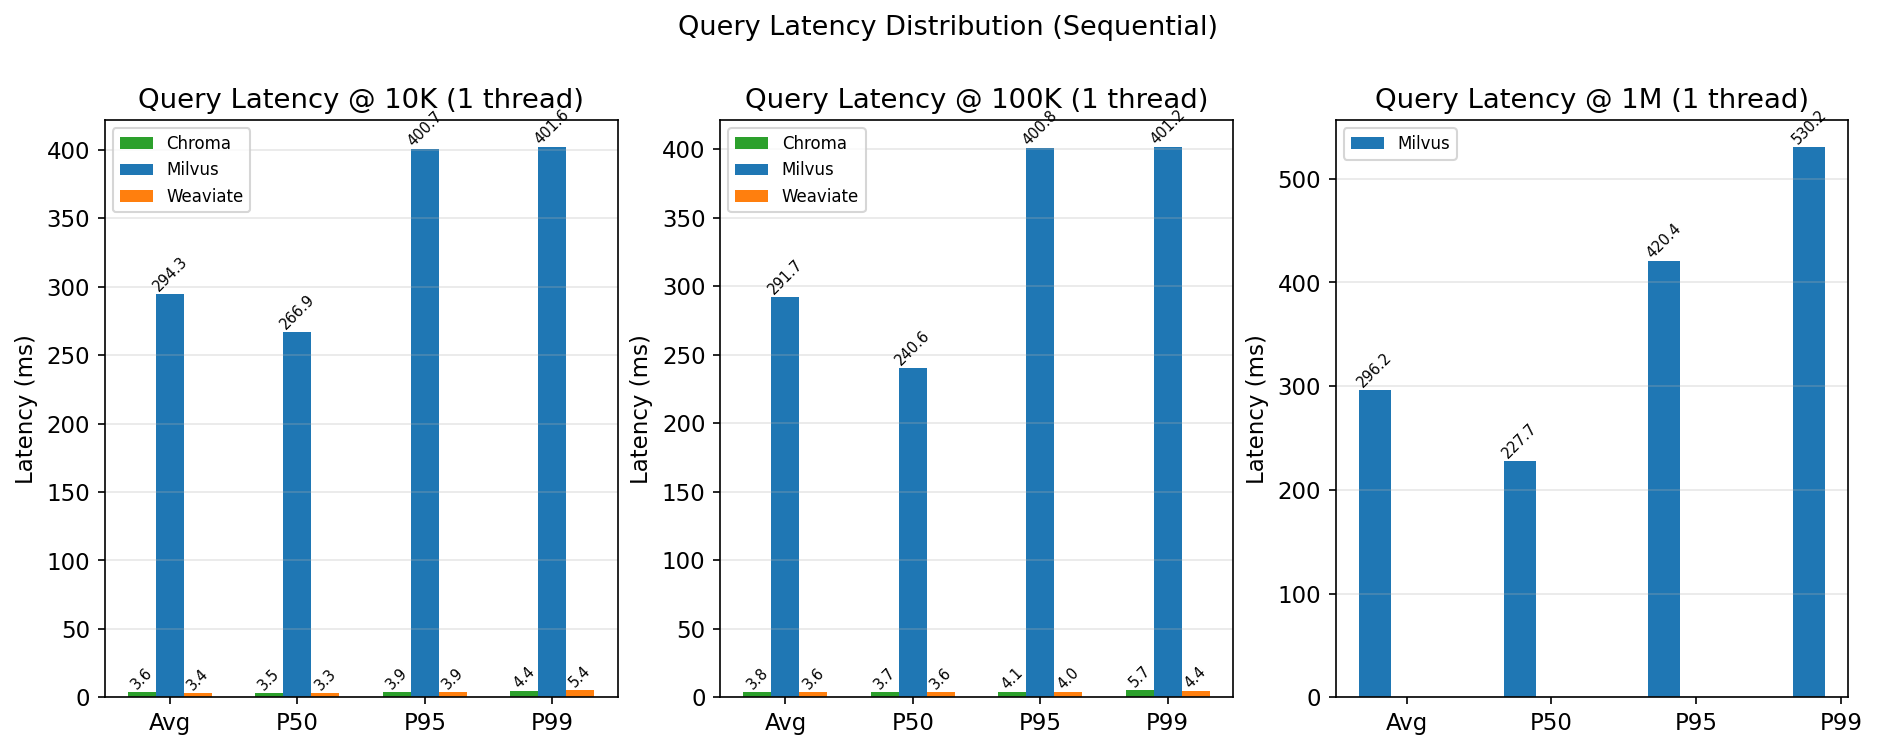
\includegraphics[width=0.95\textwidth]{figures/query_latency_sequential.png}
    \caption{Query latency (Avg, P50, P95, P99) under sequential execution. Lower is better.}
    \label{fig:latency}
\end{figure}

\textbf{Chroma and Weaviate} achieve sub-5ms average latency at both 10K and 100K due to their HNSW index ($O(\log n)$ complexity). \textbf{Milvus} exhibits 290--296 ms average latency---approximately 80$\times$ slower---due to (1) brute-force FLAT index L2 computation and (2) per-query gRPC serialization overhead. At 1M, P99 rises to 530 ms.

\subsection{Concurrency Scaling}

Figure~\ref{fig:concurrency} shows query throughput (QPS) as concurrency increases from 1 to 16 threads.

\begin{figure}[H]
    \centering
    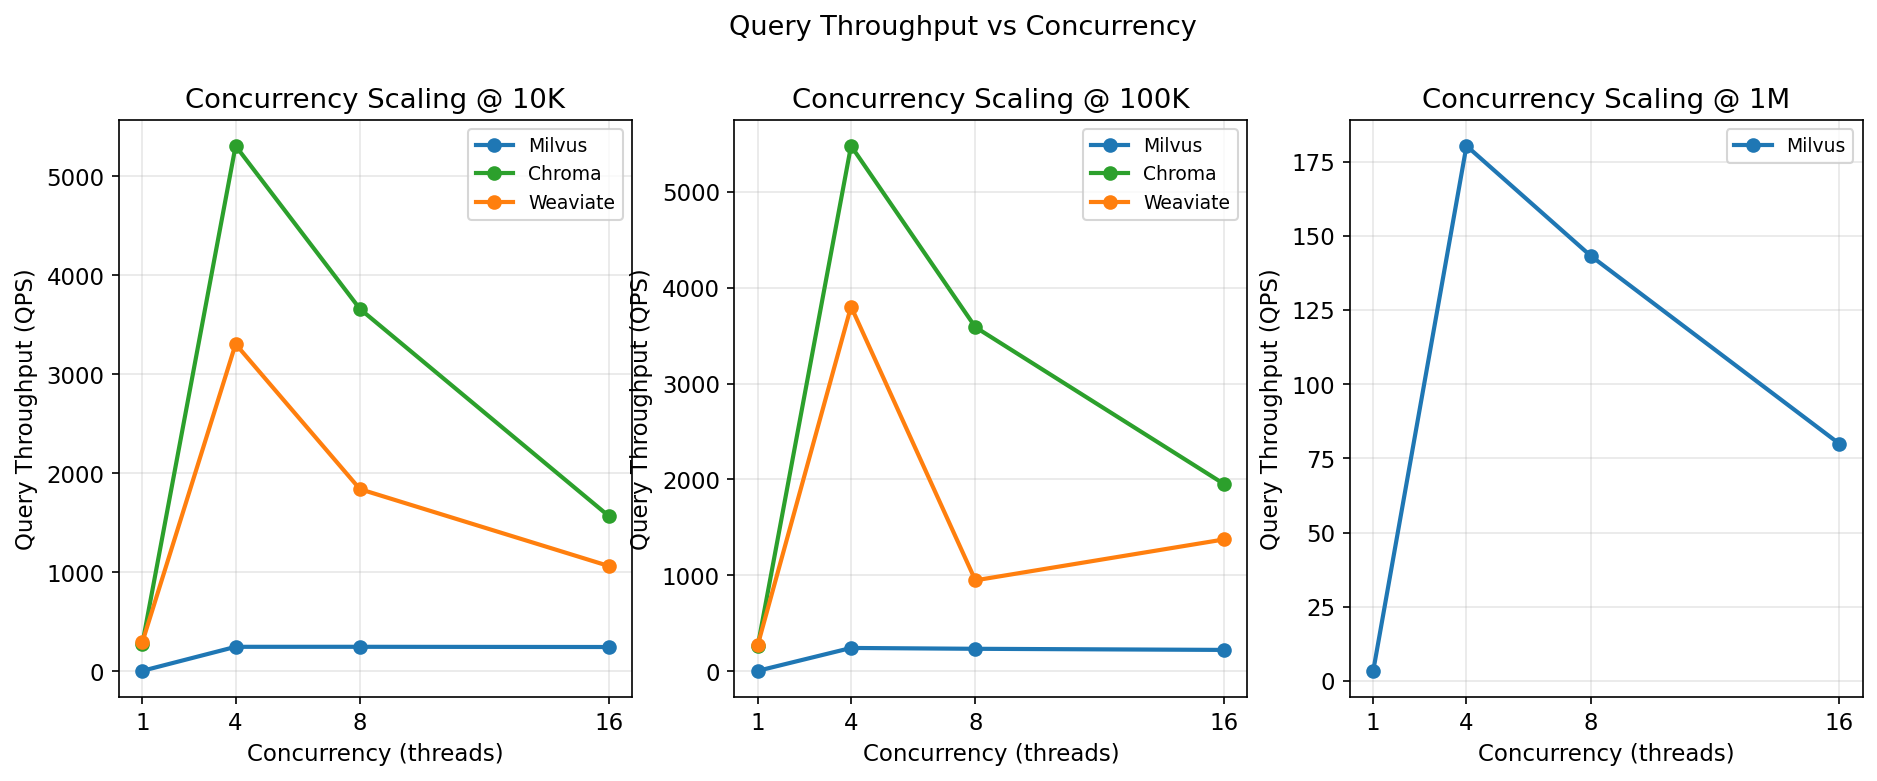
\includegraphics[width=0.95\textwidth]{figures/concurrency_scaling.png}
    \caption{Query throughput (QPS) vs.\ concurrency level. Higher is better.}
    \label{fig:concurrency}
\end{figure}

\textbf{Chroma} peaks at 4 threads (5,479 QPS at 100K), then degrades due to the Python GIL. \textbf{Weaviate} peaks similarly at 4 threads (3,803 QPS) but shows higher variance at 8--16 threads from goroutine scheduling contention. \textbf{Milvus} shows flat throughput ($\sim$242 QPS at 100K) regardless of concurrency, bottlenecked by gRPC round-trips and brute-force FLAT index on 2 vCPUs.

\subsection{Tail Latency Under Load}

Figure~\ref{fig:p95} shows how P95 latency changes under increasing concurrency.

\begin{figure}[H]
    \centering
    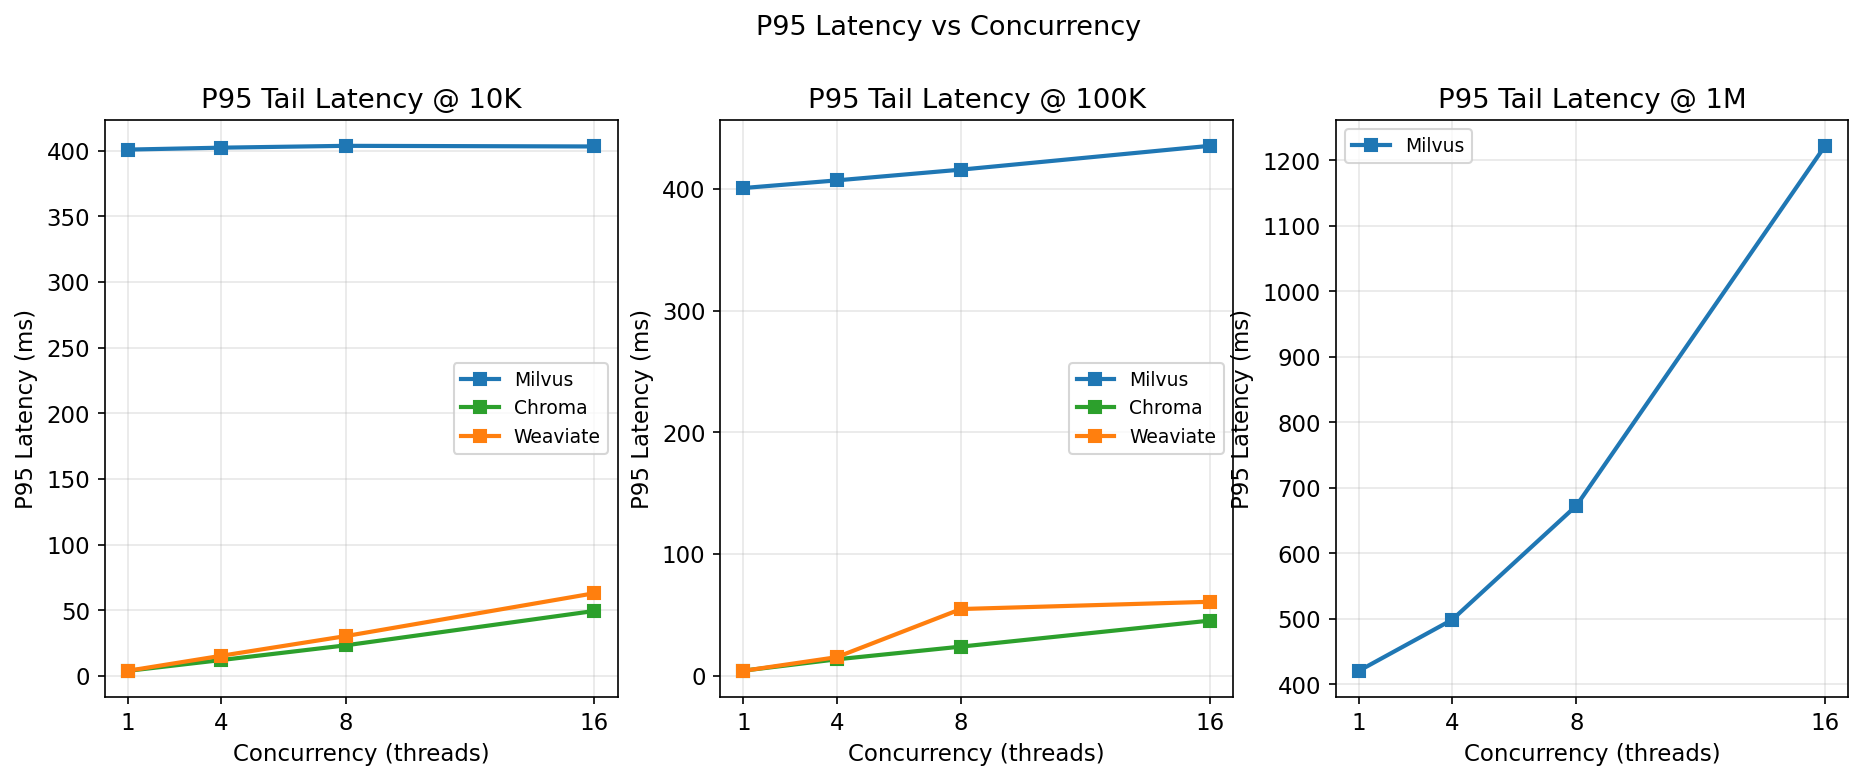
\includegraphics[width=0.95\textwidth]{figures/p95_latency_concurrency.png}
    \caption{P95 tail latency vs.\ concurrency. Lower is better.}
    \label{fig:p95}
\end{figure}

Chroma and Weaviate maintain P95 under 60~ms even at 16 threads for 10K/100K. Milvus P95 remains $\sim$400~ms at 100K but degrades to 1,222~ms at 1M/16 threads, indicating resource exhaustion.

\subsection{Memory Consumption}

Figure~\ref{fig:memory} shows system memory after ingestion. Milvus consumes 6,792 MB at 1M (3 containers), leaving only 1.2 GB for the OS. Chroma and Weaviate use 1,477--1,522 MB at 100K but exceed 8 GB during 1M ingestion, triggering the OOM killer. At 10K, all fit comfortably (741--1,007 MB).

\begin{figure}[H]
    \centering
    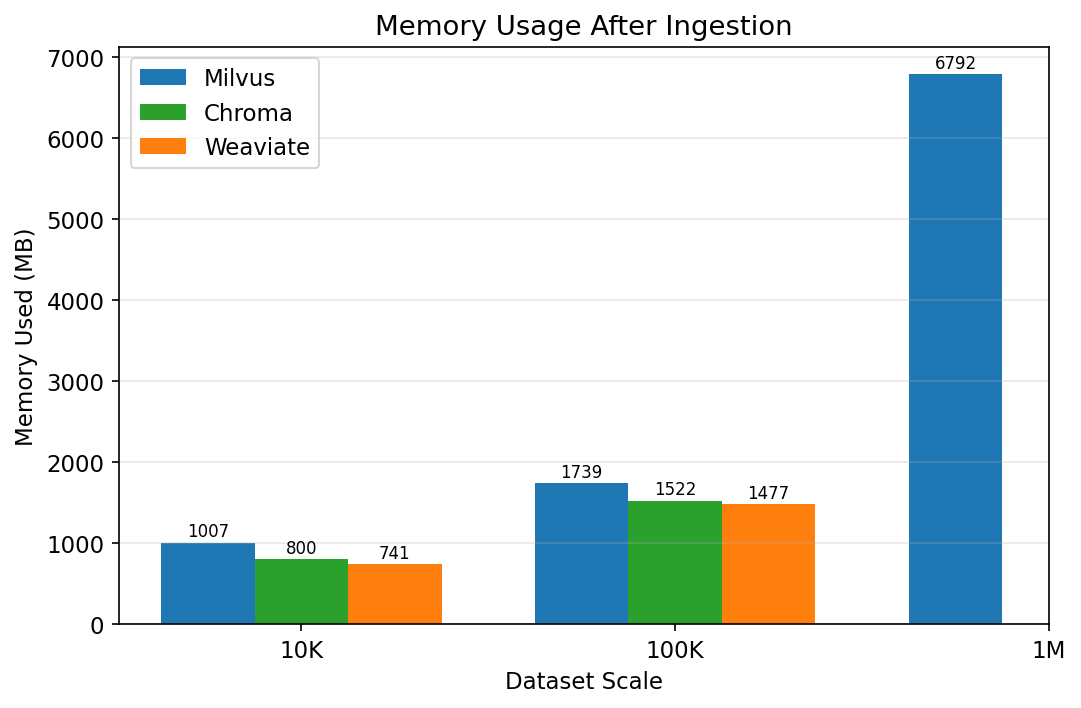
\includegraphics[width=0.78\textwidth]{figures/memory_usage.png}
    \caption{System memory usage after ingestion. Includes OS and Docker overhead.}
    \label{fig:memory}
\end{figure}

\subsection{Scalability Limits}

Table~\ref{tab:scalability} summarizes the success or failure of each database at each scale.

\begin{table}[H]
\centering
\caption{Scalability results on t2.large (8 GB RAM).}
\label{tab:scalability}
\small
\begin{tabular}{lccc}
\toprule
\textbf{Scale} & \textbf{Milvus} & \textbf{Chroma} & \textbf{Weaviate} \\
\midrule
10K   & Pass & Pass & Pass \\
100K  & Pass & Pass & Pass \\
1M    & \textbf{Pass} & Fail (OOM) & Fail (OOM / Timeout) \\
\bottomrule
\end{tabular}
\end{table}

Chroma's 1M failure is caused by its in-memory HNSW index exceeding available RAM. Weaviate fails with a \texttt{ReadTimeout} during batch ingestion, followed by the OOM killer terminating the container. Only Milvus, which offloads data to minio (disk-backed object storage), survives the 1M workload on 8 GB RAM.

% ============================================================
% 5. Cost Analysis
% ============================================================
\section{Cost Analysis}

Table~\ref{tab:tco} presents the monthly TCO for running a vector database on EC2 t2.large.

\begin{table}[H]
\centering
\caption{Monthly Total Cost of Ownership (TCO) on AWS EC2 t2.large.}
\label{tab:tco}
\small
\begin{tabular}{lrr}
\toprule
\textbf{Component} & \textbf{Specification} & \textbf{Cost (USD/month)} \\
\midrule
EC2 compute & t2.large, on-demand & \$67.74 \\
EBS storage & 30 GB gp3 & \$2.40 \\
Data transfer & $\sim$1 GB outbound & \$0.09 \\
\midrule
\textbf{Total} & & \textbf{\$70.23} \\
\bottomrule
\end{tabular}
\end{table}

The per-experiment cost is negligible: Milvus's full 3-scale benchmark (9 rounds) consumed approximately 9 minutes of EC2 time (\$0.014), Weaviate 4 minutes (\$0.006), and Chroma 2 minutes (\$0.003).

For production deployments requiring 1M+ vectors, practitioners would need at least a \texttt{t3.xlarge} (4 vCPU, 16 GB RAM, \$0.1664/hr = \$121.47/month) or \texttt{r5.large} (2 vCPU, 16 GB RAM, \$0.126/hr = \$91.98/month) to accommodate all three databases. For Milvus with its disk-backed architecture, the t2.large may suffice for up to $\sim$2M vectors with sufficient EBS.

% ============================================================
% 6. Discussion
% ============================================================
\section{Discussion}

\subsection{Deployment Guidelines}

For \textbf{prototyping with $<$100K vectors}, Chroma offers sub-4ms latency and 5,479 QPS with single-container simplicity. For \textbf{production at $>$100K}, Milvus is the only option scaling to 1M on 8 GB RAM via disk-backed storage, at the cost of higher per-query latency. \textbf{Weaviate} provides a middle ground with low-latency REST/GraphQL APIs but limited insert performance at scale.

\subsection{Threats to Validity}

The t2.large burstable instance may deplete CPU credits during long experiments. Milvus uses FLAT index while Chroma/Weaviate default to HNSW---using HNSW on Milvus would reduce its query latency. Python's GIL limits true parallelism in concurrency tests, though queries execute in database server processes. Finally, SIFT1M is a single-distribution dataset; real RAG embeddings may exhibit different patterns.

% ============================================================
% 7. Conclusion
% ============================================================
\section{Conclusion}

This paper presented VecBench-EC2, a controlled benchmark of Milvus, Chroma, and Weaviate on AWS EC2 t2.large using the SIFT1M dataset at 10K/100K/1M scales. Our experiments demonstrate that Chroma excels at small-to-medium scale with sub-4ms query latency and over 5,000 QPS under moderate concurrency, while Milvus is the only database capable of handling 1M vectors on an 8~GB instance, achieving 35,370 vec/s ingestion throughput through its disk-backed storage architecture. These findings provide actionable guidance for practitioners selecting vector databases under cloud resource and budget constraints.

% ============================================================
% References
% ============================================================
\begin{thebibliography}{10}
\bibitem{lewis2020rag}
P. Lewis et al., ``Retrieval-augmented generation for knowledge-intensive NLP tasks,'' in \textit{Proc. NeurIPS}, 2020.

\bibitem{pan2024survey}
J. Pan et al., ``Survey of vector database management systems,'' \textit{VLDB Journal}, vol. 33, pp. 1039--1068, 2024.

\bibitem{wang2021milvus}
J. Wang et al., ``Milvus: A purpose-built vector data management system,'' in \textit{Proc. ACM SIGMOD}, 2021, pp. 2614--2627.

\bibitem{chroma2024}
Chroma, ``Chroma --- the AI-native open-source embedding database,'' 2024. [Online]. Available: \url{https://www.trychroma.com/}

\bibitem{weaviate2024}
SeMI Technologies, ``Weaviate vector database,'' 2024. [Online]. Available: \url{https://weaviate.io/}

\bibitem{annbenchmarks}
M. Aum\"{u}ller, E. Bernhardsson, and A. Faithfull, ``ANN-Benchmarks: A benchmarking tool for approximate nearest neighbor algorithms,'' \textit{Information Systems}, vol. 87, 2020.

\bibitem{vectordbbench}
Zilliz, ``VectorDBBench: Open-source vector database benchmark tool,'' 2024. [Online]. Available: \url{https://github.com/zilliztech/VectorDBBench}

\bibitem{malkov2018hnsw}
Y. A. Malkov and D. A. Yashunin, ``Efficient and robust approximate nearest neighbor search using hierarchical navigable small world graphs,'' \textit{IEEE Trans. PAMI}, vol. 42, no. 4, pp. 824--836, 2020.

\bibitem{jegou2011sift}
H. J\'{e}gou, M. Douze, and C. Schmid, ``Product quantization for nearest neighbor search,'' \textit{IEEE Trans. PAMI}, vol. 33, no. 1, pp. 117--128, 2011.

\bibitem{awspricing}
Amazon Web Services, ``Amazon EC2 on-demand pricing,'' 2026. [Online]. Available: \url{https://aws.amazon.com/ec2/pricing/on-demand/}
\end{thebibliography}

% ============================================================
% Artifact Appendix (does NOT count toward page limit)
% ============================================================
\newpage
\appendix
\section*{Artifact Appendix}

\subsection*{A.1 Abstract}

This artifact contains the complete benchmark framework, Docker Compose configurations, dataset preparation scripts, and analysis tools used in this paper. All experiments can be reproduced on an AWS EC2 t2.large instance running Ubuntu 22.04.

\subsection*{A.2 Artifact Location}

\begin{itemize}[nosep]
    \item \textbf{GitHub Repository}: \url{https://github.com/doubledoubleq666-blip/VecBench-EC2}
    \item \textbf{License}: MIT
\end{itemize}

\subsection*{A.3 Requirements}

\textbf{Hardware:}
\begin{itemize}[nosep]
    \item AWS EC2 t2.large or larger (2+ vCPU, 8+ GB RAM)
    \item 30 GB EBS gp3 storage
\end{itemize}

\textbf{Software:}
\begin{itemize}[nosep]
    \item Ubuntu 22.04 LTS
    \item Docker CE 24+ with Compose v2
    \item Python 3.10+
    \item Dependencies: see \texttt{requirements.txt}
\end{itemize}

\subsection*{A.4 Setup and Installation}

\begin{verbatim}
# 1. Clone the repository
git clone https://github.com/doubledoubleq666-blip/VecBench-EC2
cd vecbench-ec2

# 2. Run environment setup (installs Docker, Python, venv)
chmod +x scripts/setup_env.sh
./scripts/setup_env.sh
# Log out and back in for Docker group, then:
source venv/bin/activate

# 3. Download and prepare dataset
python downloadDataset.py
python scripts/prepare_sift_subsets.py
\end{verbatim}

\subsection*{A.5 Running the Benchmark}

\begin{verbatim}
# Run all experiments (takes ~1 hour on t2.large)
nohup bash scripts/run_phase3_all.sh > results/phase3.log 2>&1 &

# Or run individual databases:
cd docker/milvus && docker compose up -d && cd ../..
python benchmark.py --db milvus --dataset data/processed/sift_10k.npy \
    --scale 10K --threads 1,4,8,16 --repeat 3 --num-queries 100
cd docker/milvus && docker compose down && cd ../..
\end{verbatim}

\subsection*{A.6 Generating Charts and Analysis}

\begin{verbatim}
python scripts/analyze_results.py
# Output: bench/charts/*.png and aggregated_results.csv
\end{verbatim}

\subsection*{A.7 Expected Results}

The benchmark produces CSV files in \texttt{results/} with columns for insert time, query latency percentiles, concurrency level, and system metrics. At 100K scale, expected approximate values:
\begin{itemize}[nosep]
    \item Milvus: insert $\sim$12,300 vec/s, query avg $\sim$292 ms
    \item Chroma: insert $\sim$3,877 vec/s, query avg $\sim$3.8 ms
    \item Weaviate: insert $\sim$1,722 vec/s, query avg $\sim$3.6 ms
\end{itemize}

\subsection*{A.8 File Structure}

\begin{verbatim}
vecbench-ec2/
  benchmark.py              # Main benchmark framework
  downloadDataset.py        # Download SIFT1M from HuggingFace
  requirements.txt          # Python dependencies
  docker/
    milvus/docker-compose.yml
    chroma/docker-compose.yml
    weaviate/docker-compose.yml
  scripts/
    setup_env.sh            # EC2 environment setup
    prepare_sift_subsets.py  # Generate .npy subsets
    smoke_test.py           # Connectivity verification
    collect_system_metrics.py
    run_phase3_all.sh       # Full experiment automation
    analyze_results.py      # Data analysis & charts
  bench/
    results/                # Raw CSV results
    charts/                 # Generated visualizations
  data/
    raw/                    # Original SIFT1M fvecs
    processed/              # 10K/100K/1M .npy subsets
\end{verbatim}

\end{document}
